\documentclass[11pt]{article}

\usepackage[margin=1.0in]{geometry}
%\linespread{1.5}
\usepackage{graphicx}
\usepackage{amsmath}
\usepackage{cite}

% definition of \customlabel, which is used to label supplementary figures and tables
\makeatletter
\newcommand{\customlabel}[2]{%
\protected@write \@auxout {}{\string \newlabel {#1}{{#2}{\thepage}{}{}{}}}}
\makeatother



\renewcommand{\bottomfraction}{.9}
\renewcommand{\topfraction}{.9}
\renewcommand{\textfraction}{0.1}
\renewcommand{\floatpagefraction}{.9}


\begin{document}
\title{\textbf{The relationship between dN/dS and scaled selection coefficients}}
\author{Stephanie J. Spielman$^{1}$ and Claus O. Wilke$^{1}$}
\date{}

\maketitle
\noindent
Address:\\
$^1$Department of Integrative Biology, Center for Computational Biology and Bioinformatics, and Institute of Cellular and Molecular Biology.
The University of Texas at Austin, Austin, TX 78712, USA.\\

\bigskip
\noindent
$^*$Corresponding author\\
$\phantom{^*}$Email: ??????????\\

\bigskip
\noindent Keywords: selection coefficients, $dN/dS$, natural selection, protein evolution, models of sequence evolution

\newpage
\begin{abstract}
Two measures of the strength of selection on protein coding sequences are $dN/dS$ and selection coefficients. Are the the same? Are the different? We don't know! But now we do. And they're the same. Also, stop using mechanistic codon models because parameterizing them is basically impossible.
  
\end{abstract}


\section*{Introduction}

Over the years, various methods have been used to calculate the strength of natural selection acting on protein-coding sequences. Traditionally, the focus has been on estimating the evolutionary rate ratio, $dN/dS$, the rate of nonsynonymous to synonymous substitution rates. This metric indicates how quickly a protein's constituent amino acids change, and is widely used to identify cases of positive, diversifying selection ($dN/dS > 1$) \cite{NielsenYang1998, Yangetal2000, KosakovskyPondFrost2005, Huelsenbecketal2006}. Following early counting methods for estimating $dN/dS$ (e.g. refs \cite{LWL85} and \cite{NG86}), mechanistic codon models, which assume an explicit Markov-process model of sequence evolution (see ref.~\cite{Anisimova2009} for a comprehensive review), have taken a leading role as the inference method of choice since their introduction in the 1990s \cite{GoldmanYang1994, MuseGaut1994, NielsenYang1998}. These models yield maximum likelihood estimates (MLEs) for the parameter $\omega$, which represents the quantity $dN/dS$, and have seen great success in the field of molecular evolution. 

A second class of models, known as mutation-selection-balance (MutSel) models, have emerged recently as a popular alternative to mechanistic codon models. The MutSel framework, couched firmly in population genetics theory, models the dynamic interplay between mutation and selection in a protein-coding sequence. MutSel models yield estimates of site-wise scaled selection coefficients, which indicate the extent to which natural selection favors, or disfavors, particular codons or amino acids at a given protein position. Although MutSel models were first introduced over 15 years ago \cite{HalpernBruno1998}, they have seen virtually no use due to their high computational expense. However, recently, several computationally tractable model implementations have emerged \cite{RodrigueLartillot2014,Tamurietal2014}, allowing for the first time the potential for widespread use. 


Although both mechanistic codon models and MutSel models describe the same fundamental process of protein-coding sequence evolution along a phylogeny, it is largely unknown how these two classes of models relate to one another. In particular, as these inference methods have been developed independently, it remains an open question whether or not parameter estimates from one model are comparable to those of the other model. Whether $dN/dS$ values have any correspondence with scaled selection coefficients remains an open question. Therefore, while certain rhetorical arguments may be made in favor of using one method over another, there is currently no formalized, concrete rationale to guide researchers in their methodological choices. 

Here, we formalize the relationship between mechanistic codon and MutSel models by examining the extent to which their focal parameters, $dN/dS$ and scaled selection coefficients, yield overlapping information about the evolutionary process. To this end, we derive a mathematical relationship these models' primary parameters from which one can infer $dN/dS$ values from selection coefficients alone. Using a simulation approach, we verify that $dN/dS$ values estimated using selection coefficients alone correspond precisely to $\omega$ MLEs inferred using standard mechanistic codon models. 

% MORE NEEDS TO BE WRITTEN HERE FOR SURE ONCE THE REST OF THE MS IS COMPLETE
(???)Further, we prove that, under conditions of symmetric mutation rates, this relationship holds only under regimes of purifying selection or neutral evolution ($dN/dS \leq 1$). This proof reveals that MutSel models are inherently unable to describe accurately protein evolution under a regime of positive diversifying selection, or when $dN/dS > 1$.

Moreover, our analyses incidentally have revealed certain biases inherent in the ML $\omega$ inference approach. (...)
 


\section*{Methods}

\subsection*{Sequence simulation}
We simulated protein-coding sequences as a continuous-time Markov
process \cite{Yang2006} according to the MutSel model proposed by \cite{HalpernBruno1998}. This model's instantaneous rate matrix $Q$ is given by 

\begin{equation}
Q_{ij} = \left\{ \begin{array}{rl}
              f_{ij}\mu_{ij}\kappa               &\mbox{single nucleotide transition} \\
              f_{ij}\mu_{ij}                          &\mbox{single nucleotide transversion} \\
              0                                           &\mbox{multiple nucleotide changes} \\             
         \end{array} \right.,
\end{equation} where $\mu_{ij}$ is the symmetric nucleotide mutation rate and $f_{ij}$, the fixation probability from codon $i$ to $j$, is defined as \begin{equation}f_{ij} = ln\bigg{(}\frac{\pi_j\mu_{ij}}{\pi_i\mu_{ji}}\bigg{)}\bigg{/}\bigg{(}1 - \frac{\pi_i\mu_{ji}}{\pi_j\mu_{ij}}\bigg{)},\end{equation} where $\pi_i$ is the equilibrium frequency of codon $i$.

We simulated protein-coding sequences along a 10-taxon phylogeny, with all branch lengths equal to 0.01, beginning with a root sequence selected using steady-state codon frequencies. We set a global nucleotide mutation rate of $\mu_{xy} = 10^{-6}$, and we drew a value for each simulation's $\kappa$ from $\mathcal{U} \sim (1,6)$, resulting in a fully symmetric mutation matrix. Unless otherwise stated, all simulated alignments contained 500,000 codon positions. A single evolutionary model was applied to all positions in the simulated sequences. While this lack of site-wise heterogeneity is unrealistic for real sequence evolution, it allows us to verify our derived relationship between selection coefficients and $dN/dS$ with a sufficiently sized data set.

\subsection*{Assigning scaled selection coefficients}

We simulated 100 alignments under the assumption that all synonymous codons have equal fitness (e.g. no codon bias), and a second set of 100 alignments which incorporated codon bias. For both frameworks, we generated amino acid scaled selection coefficients, $S_a$, for each simulation, by fixing one coefficient to 0 and drawing the remaining 19 values from a normal distribution $\mathcal(N)\sim(0,\sigma^2)$, where $\sigma^2 \sim U(0,4)$. Here, $\sigma^2$ effectively represents the strength of natural selection; larger values of $\sigma^2$ will correspond to greater fitness differences among amino acids, and thus more selective pressure.


For simulations without codon bias, we assigned these amino acid selection coefficients to codons such that all synonymous codons had the same scaled selection coefficient. For simulations with codon bias, we randomly selected a preferred codon for each amino acid. We then assigned the preferred codon a selection coefficient of $S_a + b$, where $b=(2)$, and we assigned non-preferred codons selection coefficients of $S_a - b/(k-1)$, where $k$ is the total number of synonymous codons for the given amino acid. In this way, the average selection coefficient for this amino acid remained unchanged, but one codon per amino acid was more selectively favored.



\subsection*{$dN/dS$ Inference}
We calculated a global $dN/dS$ for each alignment using the mathematical framework outlined in \eqref{eq:pi_i}--\eqref{eq:dS} as well using standard maximum likelihood methods. Specifically, inferred $dN/dS$ using the M0 mechanistic codon model \cite{Yangetal2000}, as implemented in the HyPhy batch language \cite{KosakovskyPondetal2005}. The M0 models uses the GY94 instantaneous rate matrix \cite{GoldmanYang1994,NielsenYang1998}, which includes the primary parameters $\omega$, $\kappa$, and equilibrium codon frequencies. As different $\kappa$ and equilibrium codon frequency parameterizations can change $\omega$ estimates \cite{YN00, Yang2006, ZhangYu2006}, we inferred $\omega$ under a variety of model parameterizations, including three $\kappa$ parameterizations ($\kappa$ fixed to 1, $\kappa$ as a free parameter, and $\kappa$ fixed to its true value), and four codon frequency specifications (equal codon frequencies,  F3x4 codon frequencies \cite{MuseGaut1994}, CF3x4 codon frequencies \cite{Pond2010} and empirical codon frequencies), ultimately resulting in 12 $\omega$ MLEs per simulated alignment. Note that we additionally verified that the system was evolving under a state-state process by verifying that the true, simulated codon frequencies were the same as the empirical codon frequencies calculated from the simulated alignment. All code used is freely available at \textbf{github}. 



\section*{Results}


\section*{Mathematical relationship between selection coefficients and omega}


We describe here how to calculate $dN/dS$ from the parameters of a MutSel model. Under the assumption that the mutational process is symmetric, e.g. $\mu_{xy}=\mu_{yx}$ for all nucleotide pairs $xy$, we can write the steady-state frequency of codon $i$ as 
\begin{equation}\label{eq:pi_i}
 \pi_i=\frac{e^{S_i}}{\sum_k e^{S_k}},
\end{equation}
where the sum in the denominator runs over all 61 sense codons \cite{SellaHirsh2005}. Here, $S_i$ is the scaled selection coefficient for codon $i$; larger $S_i$ values correspond to higher frequencies of codon $i$.

The fixation probability for a mutation from codon $i$ to codon $j$ is \cite{HalpernBruno1998,SellaHirsh2005}
\begin{equation}\label{eq:f_ij}
 f_{ij} = \frac{1-(\pi_i/\pi_j)^{1/N_e}}{1-\pi_i/\pi_j}
  \approx \frac{1}{N_e} \frac{\ln \pi_j - \ln \pi_i}{1-\pi_i/\pi_j}\,,
\end{equation}
where $N_e$ is the effective population size. Using this framework, we can calculate an evolutionary rate by summing over all substitution probabilities weighted by the frequency of the originating codon. Further, we can establish specific expressions for nonsynonymous and synonymous evolutionary rates, and then divide them in order to obtain a value for the evolutionary rate ratio $dN/dS$.

To begin, we can write the nonsynonymous rate $K_\text{N}$ as 
\begin{equation}\label{eq:KN}
  K_\text{N} = N_e \sum_i \sum_{j \in {\cal N}_i} \pi_i  f_{ij}\mu_{ij}\,,
\end{equation}
where ${\cal N}_i$ is the set of codons that are nonsynonymous to codon $i$ and differ from it by one nucleotide. To normalize $K_\text{N}$, we divide it by the number of nonsynonymous sites, which we calculate according to the mutational opportunity definition of a site \cite{GoldmanYang1994, Yang2006} as 
\begin{equation}\label{eq:LN}
  L_\text{N} = \sum_i \sum_{j \in {\cal N}_i} \pi_i \mu_{ij}\,, 
\end{equation} and thus we find that 
\begin{equation}\label{eq:dN}
  dN = \frac{K_\text{N}}{L_\text{N}}=\frac{ N_e \sum_i \sum_{j \in {\cal N}_i} \pi_i f_{ij} \mu_{ij} } {\sum_i \sum_{j \in {\cal N}_i} \pi_i \mu_{ij} }\,.
\end{equation}

Similarly, for $dS$, the synonymous evolutionary rate $K_\text{S}$ per synonymous site $L_\text{S}$, we find
\begin{equation}\label{eq:dS}
  dS = \frac{K_\text{S}}{L_\text{S}}=\frac{ N_e \sum_i \sum_{j \in {\cal S}_i} \pi_i f_{ij} \mu_{ij} } {\sum_i \sum_{j \in {\cal S}_i} \pi_i \mu_{ij} }\,,
\end{equation}
where ${\cal S}_i$ is the set of codons that are synonymous to codon $i$ and differ from it by one nucleotide substitution. The quantities $K_\text{S}$ and $L_\text{S}$ are defined as in Eqs.~\eqref{eq:KN} and \eqref{eq:LN} but summing over $j\in {\cal S}_i$ instead of $j\in {\cal N}_i$.

Equations \eqref{eq:pi_i}--\eqref{eq:dS} establish a connection between the scaled selection coefficients and the evolutionary rate ratio $dN/dS$. Moreover, we note that, if we assume that all synonymous codons have equal fitness (e.g. synonymous mutations are neutral), the synonymous fixation rate $f_{ij}= 1/N_e$ \cite{CrowKimura1970}. Under this circumstance, the value for $dS$ would reduce to 1.


\subsection*{$dN/dS$ can be accurately predicted from scaled selection coefficients}

[we refer to $dN/dS$ calculated via ssc's as derived dN/dS]

To validate our derived relationship between scaled selection coefficients and $dN/dS$, we simulated protein-coding sequences along a 10-taxon phylogeny according to a mutation-selection model framework \cite{HalpernBruno1998,SellaHirsh2005}. We simulated 100 alignments which gave equal fitness values to synonymous codons, and 100 alignments which incorporated codon bias (see Method for details). All simulations assumed a symmetric nucleotide rate matrix. For each alignment, we calculated $dN/dS$ using equations \eqref{eq:pi_i}--\eqref{eq:dS} as well as using the M0 mechanistic codon model \cite{GoldmanYang1994,NielsenYang1998,Yangetal2000}, as implemented in the HyPhy batch language \cite{KosakovskyPondetal2005}.

The relationship between $dN/dS$ calculations is shown in Figure~\ref{reg_conv}A (for simulations with no codon bias) and Figure~\ref{reg_conv}B (for simulations with codon bias), and it is clear that $dN/dS$ values derived using selection coefficients agree nearly perfectly with those inferred using standard maximum likelihood methods. Fitness differences among synonymous codons do not influence this robust relationship. Additionally, in Figure~\ref{reg_conv}C, we demonstrate convergence of $dN/dS$ estimates as the size of the data set, represented by simulated alignment length,increases. Taken together, these results demonstrate that MutSel model parameters fully encapsulate information regarding $dN/dS$, and that the results from MutSel and mechanistic codon models are in complete agreement.


\subsection*{coefficients and dn/ds relate to each other}

We can prove that codon bias is less than 1 for when there is no codon bias and mutation rates are symmetric. but if you have codon bias and asymmetric mutation rates, in trouble.
also, selection coefficients and dnds are good. when selection is stronger, dnds is lower. same goes for the bias dataset, but the effect is somewhat lessened as aa coeffs no longer are totally the same as the selection process since it;s been partitioned differently.

Moreover, as seen in Figure~\ref{reg_conv}A-B, $dN/dS$ values are always less than 1, reflecting a universal regime of purifying selection. In fact, \textbf{in SuppMat,} we prove that, when calculated using scaled selection coefficients, $dN/dS$ is necessarily always less than or equal to 1, although this proof holds only when all synonymous codons have the same fitness value. 
%This important insight reveals that, while MutSel and mechanistic codon models fully agree, their relationship only holds under conditions of purifying selection or neutral evolution. MutSel models, therefore, are inherently unable to describe protein evolution under positive, diversifying selection ($dN/dS > 1$).



\subsection*{Influence of ML model parameterizations}

The maximum likelihood $dN/dS$ estimates (the model's $\omega$ parameter) reported in the previous subsection were obtained by fixing $\kappa$ parameter in the GY94 rate matrix to its true simulated value, and specifying equal codon frequencies. However, as different model parameterizations can influence the resulting $\omega$ MLE \cite{YN00,Yang2006,ZhangYu2006}, we inferred $\omega$ according to a total of 12 distinct model parameterizations, including three parameterizations for $\kappa$ (fixed to its true value, fixed to 1, or a free parameter of the model) as well as four equilibrium codon frequency specifications (equal codon frequencies, frequencies calculated using either the F3x4 \cite{MuseGaut1994} or the CF3x4 \cite{Pond2010} estimators, or empirical codon frequencies as taken from the simulated alignment). Table~\ref{tab:mlspec} shows how the $\omega$ values estimated according to these different ML parameterizations relate to the $dN/dS$ values as calculated using equations \eqref{eq:pi_i}--\eqref{eq:dS}, specifically for the simulations without codon bias (Table S1 gives the equivalent results for simulations with codon bias).

Results in Table~\ref{tab:mlspec} yield several important insights into the behavior of mechanistic codon models. First, it is clear that these models only estimate $dN/dS$ accurately when equilibrium codon frequencies are set as equal (i.e., each codon has a frequency of $1/61$). Second, the F3x4 and CF3x4 frequency estimators perform nearly identically to one another (p=0.54), yielding $\omega$ estimates with weak, negative correlations with the $dN/dS$ derived from selection coefficients. Finally, when empirical codon frequencies are used, $\omega$ estimates have a moderately strong, negative correlation with derived $dN/dS$ values. In other words, as the ML codon frequency parameters were more and more tailored to the given data set, $\omega$ MLEs decreased in accuracy. In fact, the negative correlations observed for the latter three frequency specifications actually reflect strongly overestimated $\omega$ MLEs; indeed, when empirical frequencies were specified (along with $\kappa$ fixed to its true value), $\omega$ estimates were universally above 1.  Figure~\ref{reg_fspec} displays regressions between derived and ML inferred $\omega$ values across the equal, F3x4, and empirical codon frequency specifications with $\kappa$ fixed to its true value ($dN/dS$ regression plots for all ML parameterizations are shown 
for simulations without codon bias in Figure~\ref{fig:reg_allspecs_nobias} and for simulations with codon bias in Figure~\ref{fig:reg_allspecs_bias}).

However, it is interesting to note that, while ML yields the most accurate $\kappa$ estimates when equal codon frequencies are specified, all frequency specifications yield $\kappa$ estimates which correlate fairly well with the true, simulated $\kappa$ values. Thus, the ML model's ability to accurately estimate $\kappa$ appears much more robust to codon frequency specifications is than its ability to estimate $\omega$. Regression plots displaying the relationship between true $\kappa$ values and $\kappa$ MLEs are shown in Figures~\ref{fig:reg_kappa_nobias} and ~\ref{fig:reg_kappa_bias}, for simulations without and with codon bias, respectively.


LIMITING CASES - when sd=0,basically you have neutral evolution. ml actually seems able to pick up on the neutral, but when fitness differences among amino acids are bigger, you have more problems.

We additionally examined whether frequency parameterization error was consistent across selective strengths, as seen in Figure~\ref{stddev_error}. We found that for no codon bias, interaction effect. In general, as amino acid fitness differences increased, error increased, but the slope was much higher for F3x4 and even higher for F61. This is likely because F3x4 results in flatter distributions than the F61. Importantly, error is minimized across all freqspecs when sd approaches 0. This is the case of neutral evolution, so selection pressure is minimal, and thus freqspec matters much less because selection is not a strong and thus not really represented by those parameters.
In codon bias, we did not detect a sig interaction effect. This also makes sense since selection doesn't entirely scale with amino acids. Plus, we see that error is not minimized at sd=0, because this isn't neutral! codons have diff fitness values. 


\subsection*{Discussion}
The oldest and most-widely used method to infer selection pressure in protein-coding genes calculates calculates the ratio of non-synonymous ($dN$) to synonymous ($dS$) substitution rates $dN/dS$ to identify sites that experience negative selection ($dN/dS<1$), sites that evolve neutrally ($dN/dS\approx1$), and sites that experience positive diversifying selection ($dN/dS>1$). By contrast, MutSel models estimate scaled selection coefficients, either for individual amino acids,\cite{HalpernBruno1998,NielsenYang2008,Rodrigueetal2010,Tamurietal2012,Tamurietal2014}, for codons \cite{YangNielsen2008}, or for both. Thus, while mechanistic codon models describe the how quickly a protein's constituent amino acids change, MutSel models calculate the strength of natural selection operating on the specific amino-acid changes.  

Until now, however, it has been an open question how these two modeling frameworks relate to one another. Some have argued that MutSel models, given their firm grounding in population genetics theory and specific attention to site-specific amino acid fitness differences, offer a more fine-grained approach to studying protein evolution than do mechanistic codon models \cite{HalpernBruno1998,Rodrigueetal2010}. Recent phylogenetic studies have also demonstrated that evolutionary models which explicitly consider amino acid fitness values offer dramatic improvements over other models, including mechanistic codon models, suggesting that MutSel models may more accurately represent the process of coding-sequence evolution \cite{Bloom2014a, Bloom2014b}. 

Here, we have derived a formal mathematical relationship between the quantities $dN/dS$ and scaled codon selection coefficients, the primary parameters of mechanistic codon and MutSel models, respectively. Through a simulation approach, we find that these two models are in full agreement, and that the value for $dN/dS$ can be precisely calculated from selection coefficients alone.

Our results rest on the key assumptions that the protein sequence is evolving under steady-state, or equilibrium, conditions, and the nucleotide mutation rates are symmetric (e.g. $\mu_{xy} = \mu_{yx}$). The first assumption recapitulates the population genetics theory behind MutSel models, which assume that selection coefficients remain constant over the phylogeny, and therefore the protein is evolving along a static fitness landscape \cite{HalpernBruno1998,Rodrigueetal2010,Tamurietal2012}. We make the latter assumption of symmetric mutation rates because it allows us to derive precise quantities for equilibrium codon frequencies from selection coefficients, according to theory relating statistical physics to evolutionary biology under steady-state conditions \cite{SellaHirsh2005,deVladar2011}. These frequency calculations are non-trivial in cases of asymmetric mutation rates (e.g. mutational which generate nucleotide compositional bias), and therefore merit further study. Regardless, the mathematical relationship between selection coefficients and $dN/dS$ in equations \eqref{eq:f_ij} - \eqref{eq:dS} should hold under any mutational framework.

The equivalency between selection coefficients and $dN/dS$ values we have demonstrated is robust to differences in synonymous codon fitnesses. However, it is important to note that our implementation of codon bias explicitly assumed that frequency differences among synonymous codons resulted from fitness differences alone. In other words, the sole source of codon bias in our simulations was selection, not mutation. This implementation might not be entirely biologically realistic, as both mutational and selective forces likely contribute to codon bias in real genomes \cite{Blumer1991, Duret2002, HershbergPetrov2008, PlotkinKudla2010}. However, the key finding that we present is that fitness differences among synonymous codons do not affect the robust mathematical equivalency between scaled selection coefficients and $dN/dS$. 

Incidentally, our study recovered that mechanistic codon models can produce strongly biased inferences when parameters are incorrectly specified. In particular, $\omega$ MLE values only corresponded to the true $dN/dS$ value when the equilibrium codon frequency parameters were specified as equal (e.g. each codon had an equilibrium frequency of $1/61$). Alternatively, 
 the more common approaches of using empirical codon frequencies (also known as the F61 estimator \cite{GoldmanYang1994}) or frequency estimators such as F3x4 \cite{MuseGaut1994} and CF3x4 \cite{Pond2010} always yielded strongly dramatically inflated $\omega$ MLEs. 

We explain this phenomenon by recognizing that the rationale for including codon frequency parameters in mechanistic codon  models is to account for unequal nucleotide frequencies specifically caused by mutational and not selective forces \cite{YN00, Yang2006}. The proper values for these parameters, then, should be the codon frequencies which would exist \textit{in the absence of natural selection}. This approach is the only way to ensure that $\omega$ is the sole model parameter which contains information about natural selection. Otherwise, the $\omega$ parameter will no longer represent the true $dN/dS$ evolutionary rate ratio.

Moreover, frequency estimators such as F3x4 and CF3x4, which use positional nucleotide frequencies to calculate codon frequencies, must make the implicit assumption that observed unequal base frequencies result from biased mutation rates.
This assumption, however, may not be fully justified. Indeed, our simulated alignments featured a wide array of nucleotide compositions, with GC-contents ranging from 0.22-0.79. Given that we simulated sequences according to a symmetric mutation matrix, all compositional biases in our data sets resulted entirely from natural selection favoring particular codons, not by any bias towards unequal base frequencies. Therefore, the proper equilibrium frequency parameterization for our alignments was indeed equal codon frequencies, which would be expected in the absence of natural selection and when mutation rates are symmetric. 

These results emphasize that it is crucial to parameterize mechanistic codon models properly. Indeed, their primary parameter $\omega$ will only truly represent $dN/dS$ when all other parameters are properly specified. If codon frequencies are not properly specified, which we suspect is the case in most analyses, then the $\omega$ MLEs are virtually meaningless and do not represent selective pressure. Therefore, we contend that there is hardly ever a justification to specify empirical codon frequencies, also known as the F61 frequency estimator \cite{GoldmanYang1994}, as natural selection has clearly produced the observed frequencies. Unfortunately, the F61 frequencies are the default parameterization in the widely-used PAML software's codeml implementation \cite{Yang2007}, so we strongly recommend that users take great care when using this package.
In addition, the only robust way to ensure that codon frequencies are properly specified is through experimentally calculating mutation rates. Luckily, this data already exists for a variety of taxa, including \textbf{mutation citations}.  We recommend that, if experimental data is absent, users err on the side of caution and specify equal codon frequencies to reduce the possibility of false positives.


Finally, we contend that this methods presented in this paper reveal a promising future avenue for methodological benchmarking. Typically, researchers assess the performance of a given inference framework through simulations which adhere to the underlying model's assumptions. However, this strategy can only confirm that inference methods are behaving as expected; it cannot confirm that the underlying model accurately represents the evolutionary process. Instead, we suggest an alternate approach to benchmark inference methods, and indeed evolutionary models: assessing the extent to which distinct models agree may serve as a novel, robust strategy to determine the accuracy of different modeling frameworks.


\subsection*{Still working on placement}
This relationship holds only if the protein evolves accordingly to a strictly steady-state process, otherwise known as purifying selection. Alternatively, under non-equilibrium conditions, (e.g. positive selection, when $\omega > 1$), MutSel models are inherently unable to describe protein evolution. These findings have important implications for when the use of each model is justified; if positive selection has occurred along the protein's evolutionary trajectory, MutSel models will likely yield spurious results. This proof, however, only holds when mutation rates are symmetric and when synonymous codons have equal fitnesses. 

Moreover, results obtained when fitness differences among synonymous codons were considered raise an additional issue with $dN/dS$; even though all sequences were simulated according to a strictly steady-state process, these sequences frequently featured $dN/dS$ values greater than 1. Indeed, our derivation of $dN/dS$ from selection coefficients shows that, when fitness differences exist among synonymous codons, $dN/dS$ need not be less than 1. In contrast, the most extreme case of codon bias, in which only a single codon per amino acid is selectively tolerated, the number of synonymous sites $L_\text{S} = 0$, and thus the value for $dN/dS$ approaches infinity. This finding seems paradoxical to classic interpretations of $dN/dS >1$. Typically, these values are viewed as hallmarks of positive or diversifying selection, which is assumed to occur when the protein sequence experiences strong selective pressure to change its constituent amino acids. Positive selection, therefore, necessarily implies that the protein does not evolve at equilibrium, but rather a shift in selective constraint caused new amino acids to be favored. 


However, one must also recognize that the contention that $dN/dS > 1$ represents positive selection assumes that synonymous substitutions are selectively neutral, which is clearly not the case when codon bias exists. Therefore, it is entirely possible that estimates of positive selection as inferred via $dN/dS$ estimates in species with high levels of codon bias, such as many bacterial, \textit{Drosophila}, or certain mammalian species \cite{Duret2002, Chamaryetal2006, HershbergPetrov2008, PlotkinKudla2010}, may not be true cases of positive selection, but rather simply signals of strong codon bias.


However, the calculations here necessitate that the protein is evolving according to a strictly equilibrium process, which seems paradoxical to having positive selection. In other words, even if the protein is evolving according to a static fitness landscape, sufficient levels of codon bias may yield values for $dN/dS$ which are well above 1. Thus, it seems as though what is classically termed positive selection can result simply from strong synonymous fitness differences.
 







\clearpage
\newpage
\bibliographystyle{plos2009}
\bibliography{bibliography}	

\clearpage
\newpage

\begin{table}[htbp]
\caption {\label{tab:mlspec}Effect of ML parameterizations on inference.}
\begin{tabular}{c c c c c c}
\hline\noalign{\smallskip}
\multicolumn{1}{l}{Codon frequencies} & \multicolumn{1}{l}{$\kappa$ parameterization} & \multicolumn{1}{l}{$dN/dS$ correlation} &\multicolumn{1}{l}{$dN/dS$ error} & \multicolumn{1}{l}{$\kappa$ correlation} &\multicolumn{1}{l}{$\kappa$ error} \\
\noalign{\smallskip}\hline\noalign{\smallskip}
Fequal & True & 1 & 0.015 &   &   \\ 
Fequal & Free & 0.998 & 0.042 & 0.829 & 0.151 \\ 
Fequal & 1 & 0.986 & 0.198 &   &   \\ 
\hline\noalign{\smallskip}
F3x4 & True & 0.019 & 8.277 &   &   \\ 
F3x4 & Free & -0.013 & 8.383 & 0.477 & 0.269 \\ 
F3x4 & 1 & 0.002 & 5.825 &   &   \\ 
\hline\noalign{\smallskip}
CF3x4 & True & 0.015 & 8.252 &   &   \\ 
CF3x4 & Free & -0.015 & 8.352 & 0.476 & 0.276 \\ 
CF3x4 & 1 & -0.008 & 5.782 &   &   \\ 
\hline\noalign{\smallskip}
F61 & True & -0.522 & 56.495 &   &   \\ 
F61 & Free & -0.557 & 46.346 & 0.828 & 0.231 \\ 
F61 & 1 & -0.522 & 38.668 &   &   \\ 
\noalign{\smallskip}\hline\noalign{\smallskip}
\end{tabular}
\newline
Codon frequency specifications were either set as equal (1/61 per codon), calculated from the F3x4 estimator \cite{MuseGaut1994}, calculated from the CF3x4 estimator \cite{Pond2010}, or set equal to the simulated alignment's empirical frequencies. $\kappa$ was specified as either a fixed value, its true simulated value or 1, or as a free parameter of the model. Correlations given are between the ML $\omega$ estimate and our derived $\omega$ values. Error refers to the mean absolute error between these two $\omega$ estimates. Similar values for $\kappa$ are shown for those inferences where $\kappa$ was a free parameter of the model. Note that all is significant.
\end{table}	
	

\begin{figure*}[H]
\centerline{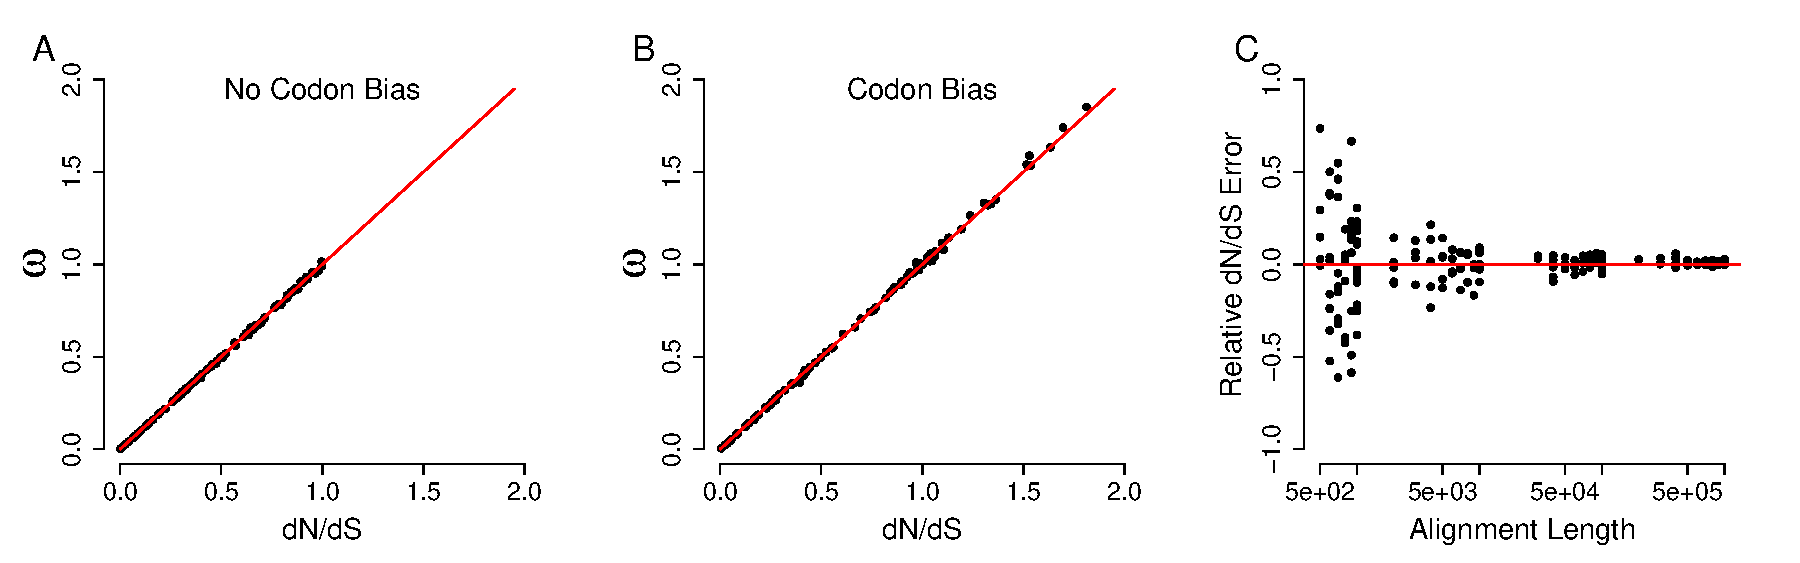
\includegraphics[width=6in]{figures/MainText/regression_convergence.pdf}}
\caption{\label{reg_conv} Relationship works exceedingly well. Left panel shows 100 points, each of which corresponds to single simulation. Note that here the ml inference is shown for equal codon frequency specs and kappa fixed to true value (a similar plot for free kappa is shown in suppfigs, but results are qualitatively identical.) Right panels shows convergence of omega values as data set size (represented as simulated alignment length) increases. The y-axis indicates relative error of the ML $dN/dS$ estimates, and the x-axis indicates sequence length on a log-scale. As the sequence length, or the data set size, increases, the two $dN/dS$ estimates converge to the same value. }
\end{figure*}


\bigskip
\begin{figure*}[H]
\centerline{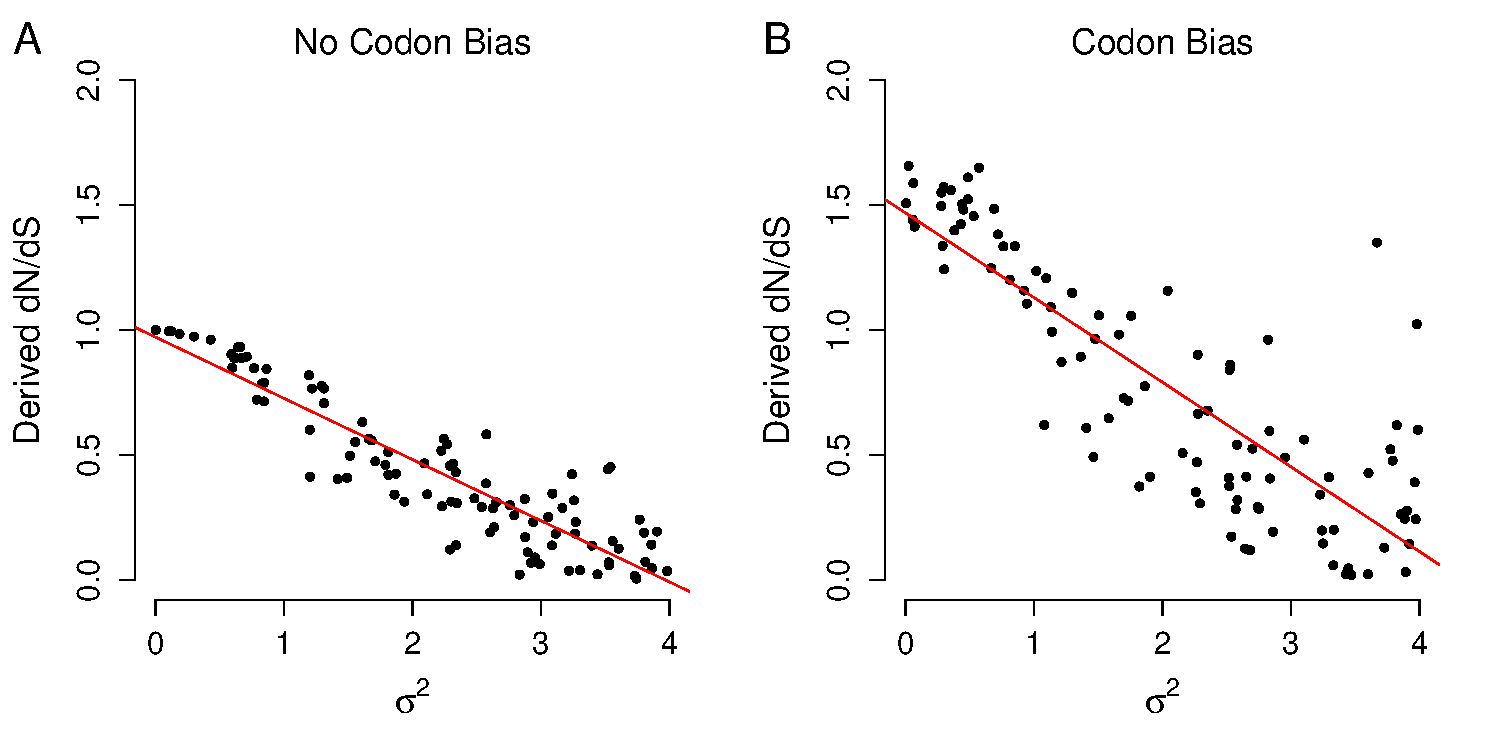
\includegraphics[width=6in]{figures/MainText/stddev_vs_dnds.pdf}}
\caption{\label{stddev_dnds} ssc's (selection strength) scales well with dnds but the strength of the relationship diminishes with codon bias as synonymous now have fitness differences, so dnds is less of a reliable indicator of selection strength.}
\end{figure*}


\bigskip
\begin{figure*}[H]
\centerline{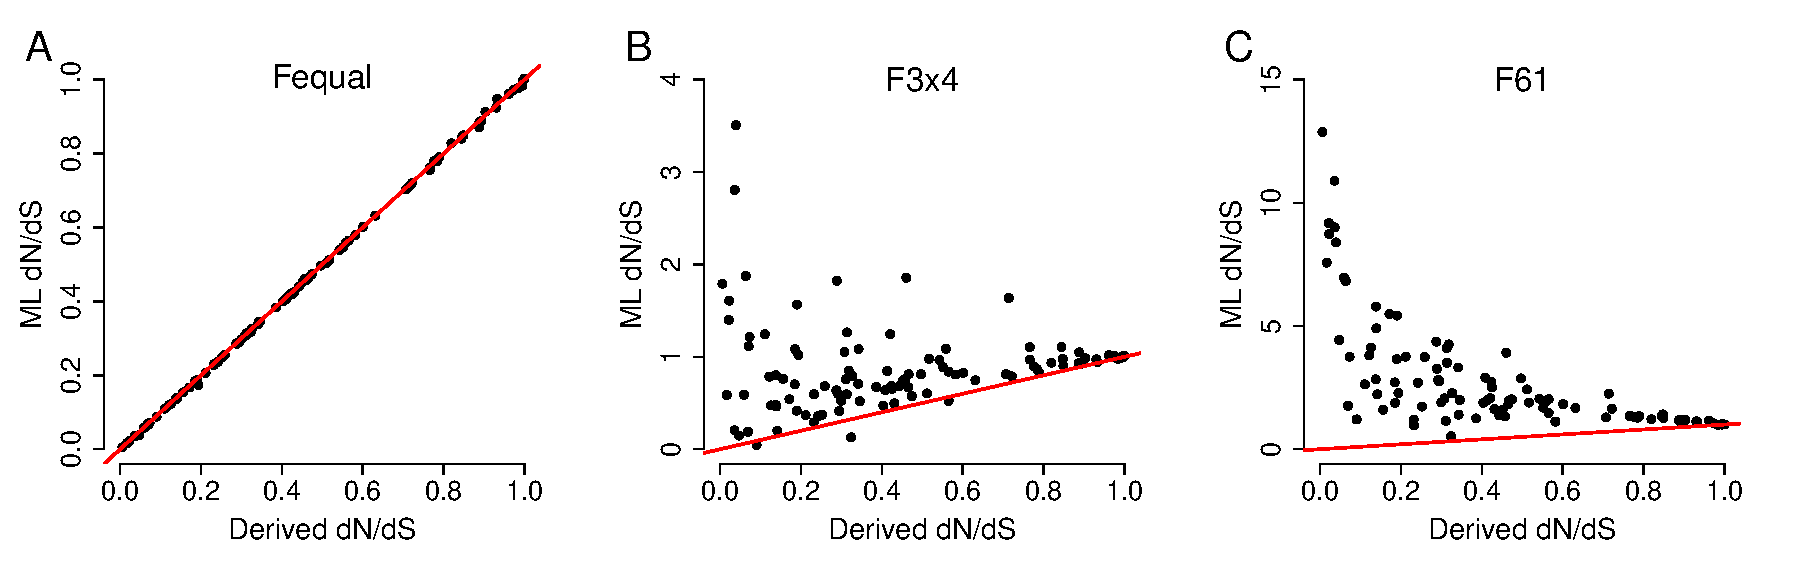
\includegraphics[width=6in]{figures/MainText/regression_omega_nobias.pdf}}
\caption{\label{reg_fspec} Issues with frequency specifications abound. In each plot, red line indicates 1:1 agreement, so note the y-axis differences. Relationship between omega values only really exists when equal codon frequencies are specified. When f3x4 or true freqs used, there is the potential to end up with dramatically inflated values. cf3x4 not shown because its results are statistically the same as f3x4.}
\end{figure*}


\bigskip
\begin{figure*}[H]
\centerline{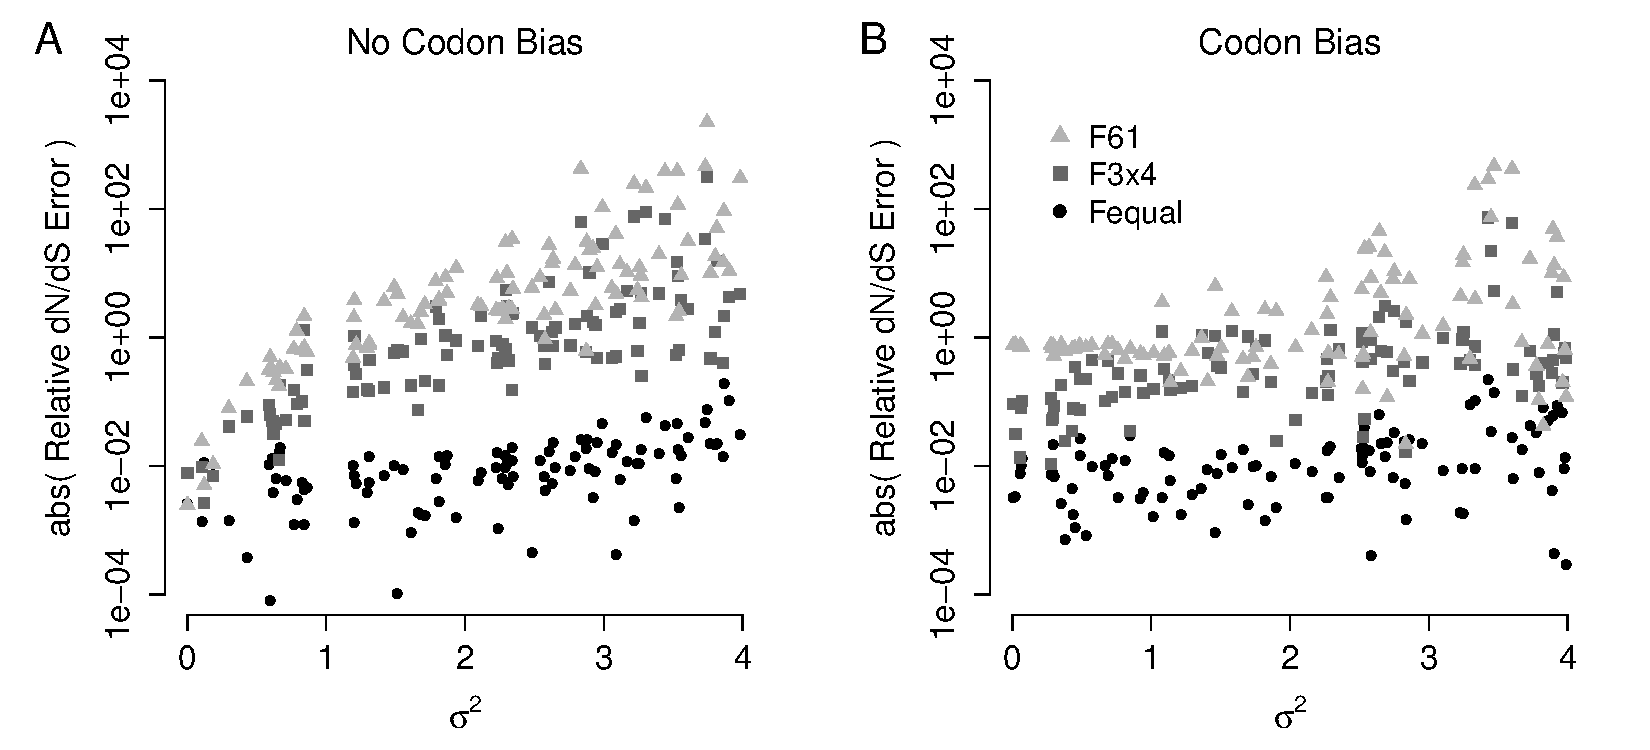
\includegraphics[width=6in]{figures/MainText/stddev_vs_error.pdf}}
\caption{\label{stddev_error} Interaction detected in no codon bias but none in the codon bias dataset.  Xaxis is stddev, Yaxis is logscale absolute value of relative error.}
\end{figure*}



\clearpage
\newpage

\section*{Supplementary Figures and Tables}

\begin{table}[htbp]
\customlabel{tab:tabS1}{tabS1}
\begin{tabular}{c c c c c c}
\hline\noalign{\smallskip}
\multicolumn{1}{l}{Codon frequencies} & \multicolumn{1}{l}{$\kappa$ parameterization} & \multicolumn{1}{l}{$dN/dS$ correlation} &\multicolumn{1}{l}{$dN/dS$ error} & \multicolumn{1}{l}{$\kappa$ correlation} &\multicolumn{1}{l}{$\kappa$ error} \\
\noalign{\smallskip}\hline\noalign{\smallskip}
Fequal & True & 1 & 0.02 &   &   \\ 
Fequal & Free & 0.971 & 0.105 & 0.699 & 0.262 \\ 
Fequal & 1 & 0.974 & 0.263 &   &   \\ 
\hline\noalign{\smallskip}
F3x4 & True & 0.646 & 2.134 &   &   \\ 
F3x4 & Free & 0.552 & 2.342 & 0.212 & 0.774 \\ 
F3x4 & 1 & 0.597 & 1.847 &   &   \\ 
\hline\noalign{\smallskip}
CF3x4 & True & 0.642 & 2.105 &   &   \\ 
CF3x4 & Free & 0.553 & 2.316 & 0.212 & 0.765 \\ 
CF3x4 & 1 & 0.581 & 1.845 &   &   \\ 
\hline\noalign{\smallskip}
F61 & True & -0.591 & 19.067 &   &   \\ 
F61 & Free & -0.281 & 27.714 & 0.315 & 0.927 \\ 
F61 & 1 & -0.56 & 12.272 &   &   \\ 
\noalign{\smallskip}\hline\noalign{\smallskip}
\end{tabular}
\newline
Results from runs with codon bias. Codon frequency specifications were either set as equal (1/61 per codon), calculated from the F3x4 estimator \cite{MuseGaut1994}, calculated from the CF3x4 estimator \cite{Pond2010}, or set equal to the simulated alignment's empirical frequencies. $\kappa$ was specified as either a fixed value, its true simulated value or 1, or as a free parameter of the model. Correlations given are between the ML $\omega$ estimate and our derived $\omega$ values. Error refers to the mean absolute error between these two $\omega$ estimates. Similar values for $\kappa$ are shown for those inferences where $\kappa$ was a free parameter of the model. Note that all is significant.
\end{table}	

\clearpage


\centerline{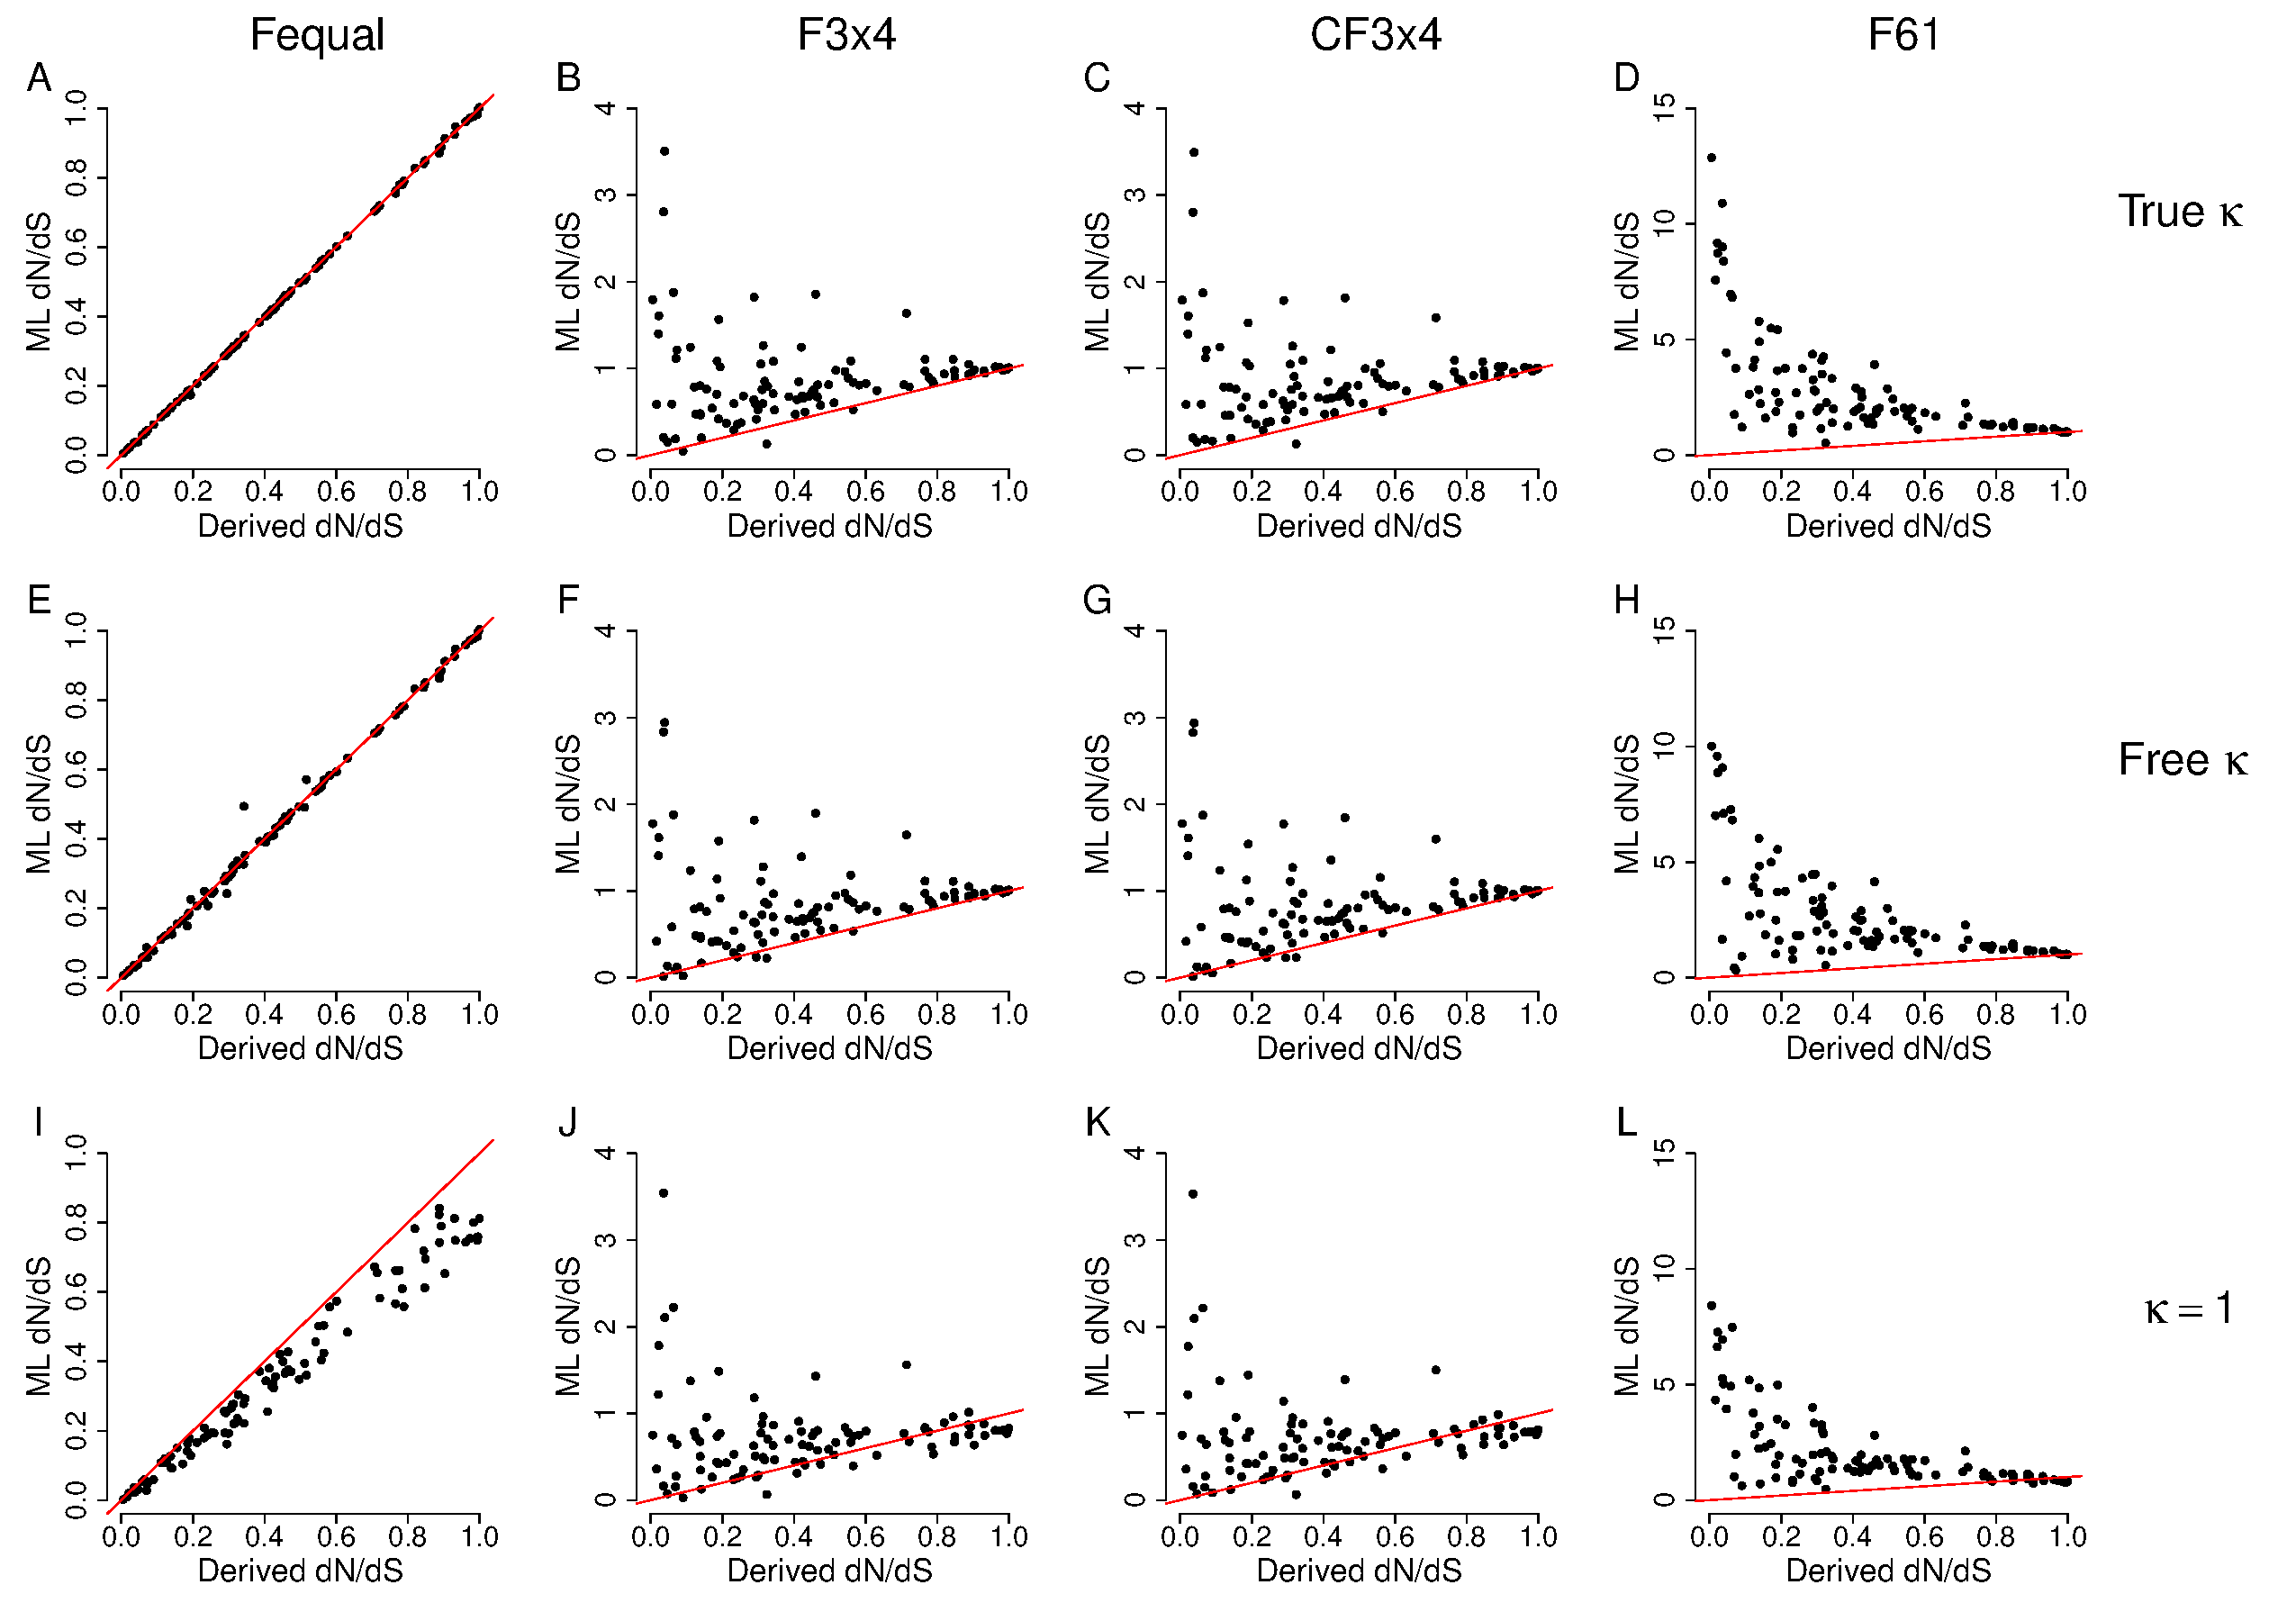
\includegraphics[width=7in]{figures/SI/regression_omega_nobias.pdf}}
\noindent \textbf{Fig. S1} Omega regression for all ML parameterizations, without codon bias.
\customlabel{fig:reg_allspecs_nobias}{S1}

\clearpage


\centerline{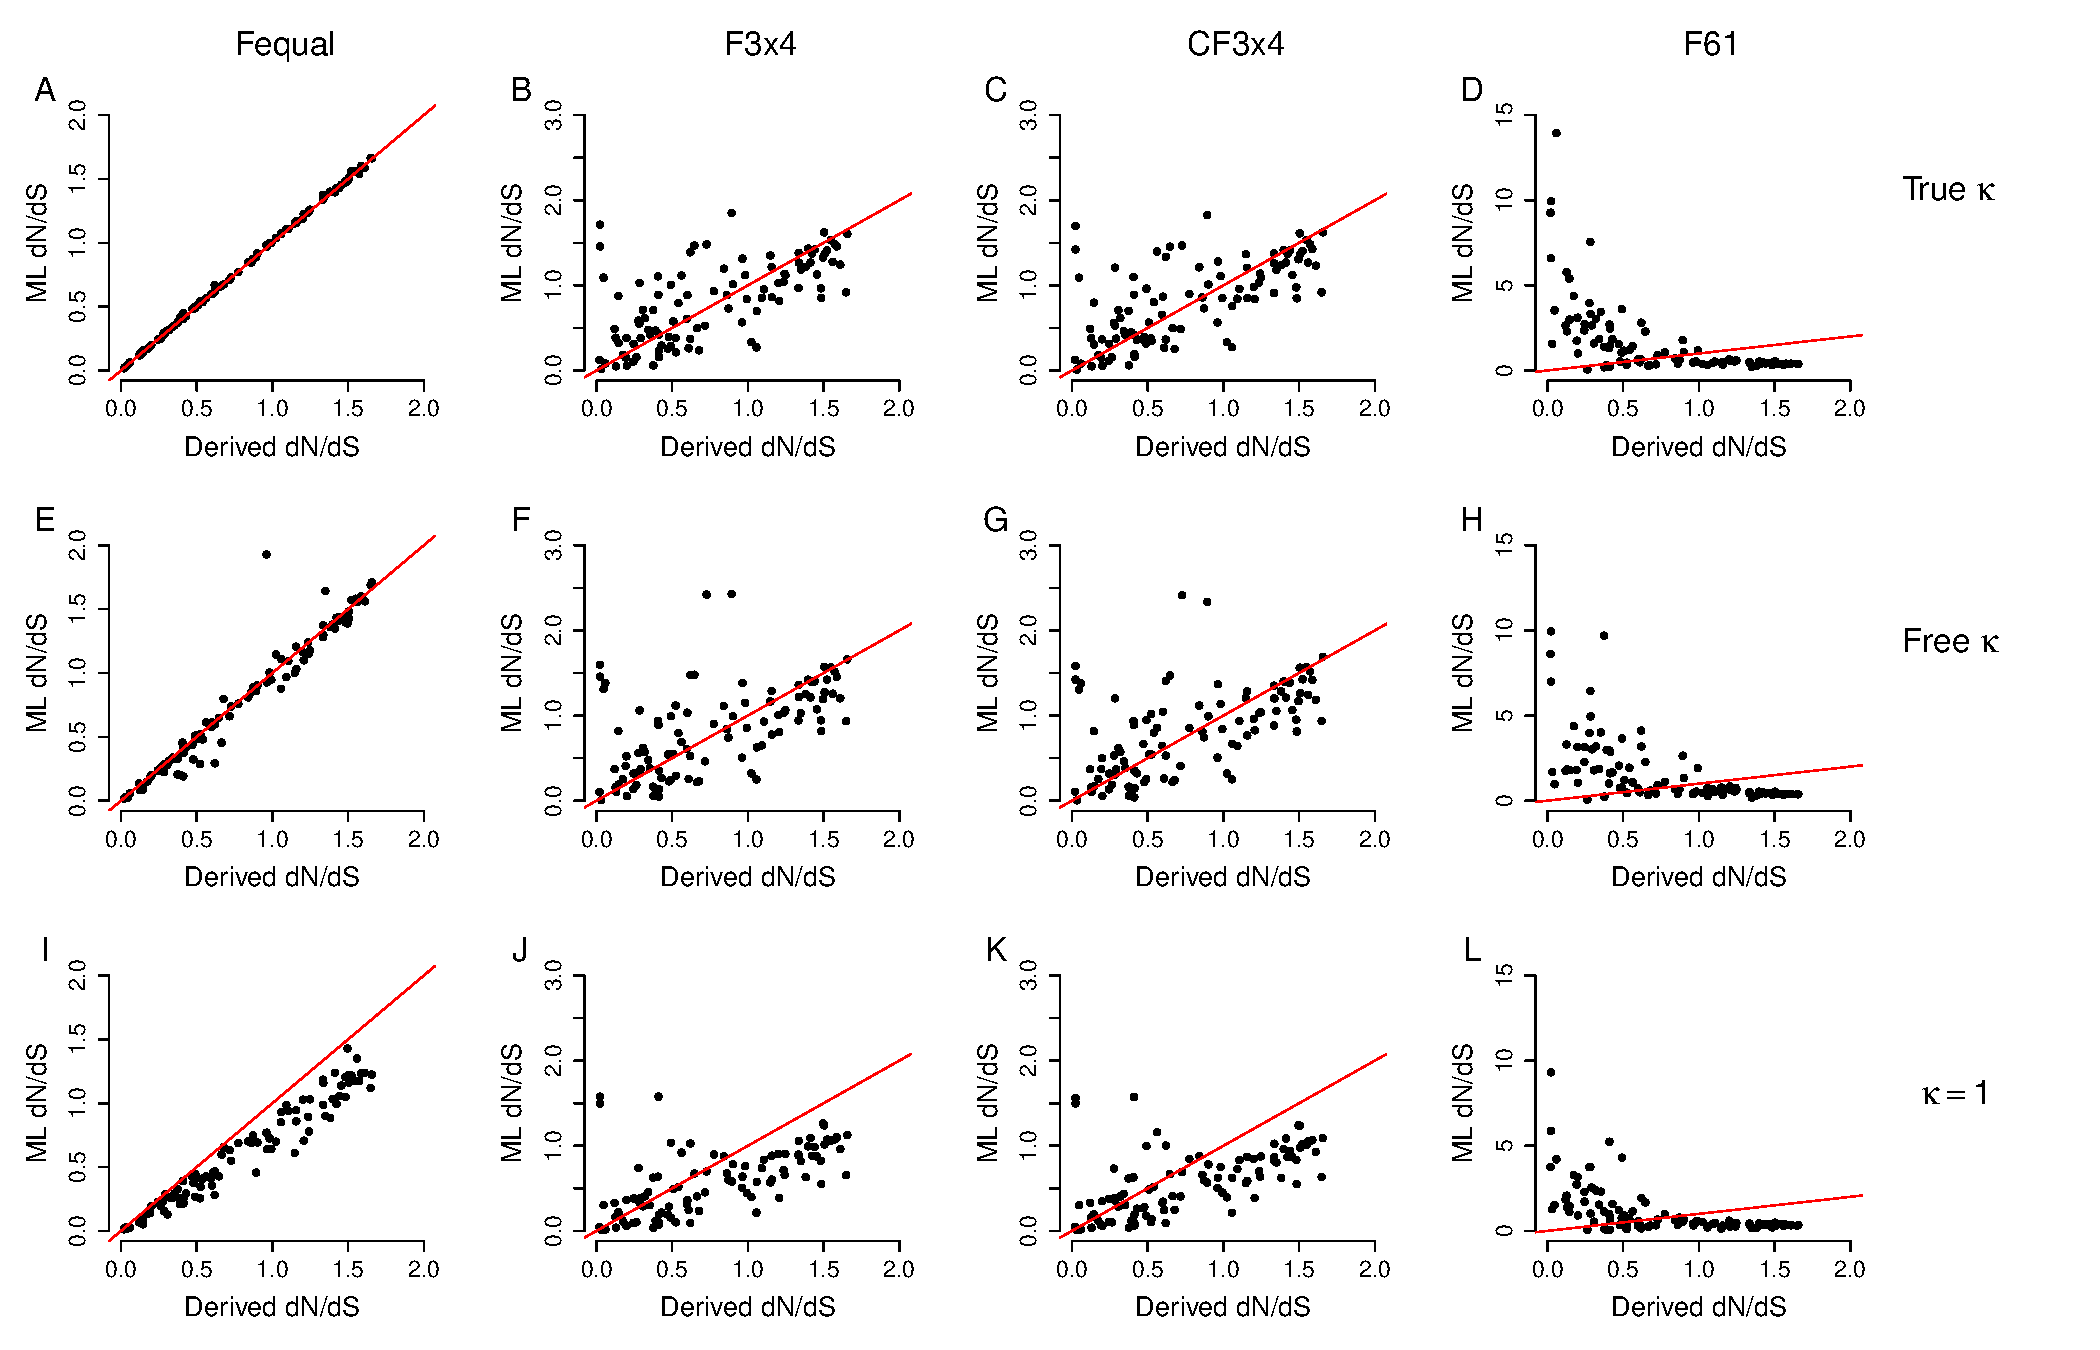
\includegraphics[width=7in]{figures/SI/regression_omega_bias.pdf}}
\noindent \textbf{Fig. S2} Omega regression for all ML parameterizations, with codon bias.
\customlabel{fig:reg_allspecs_bias}{S2}

\bigskip
\bigskip
\bigskip


\centerline{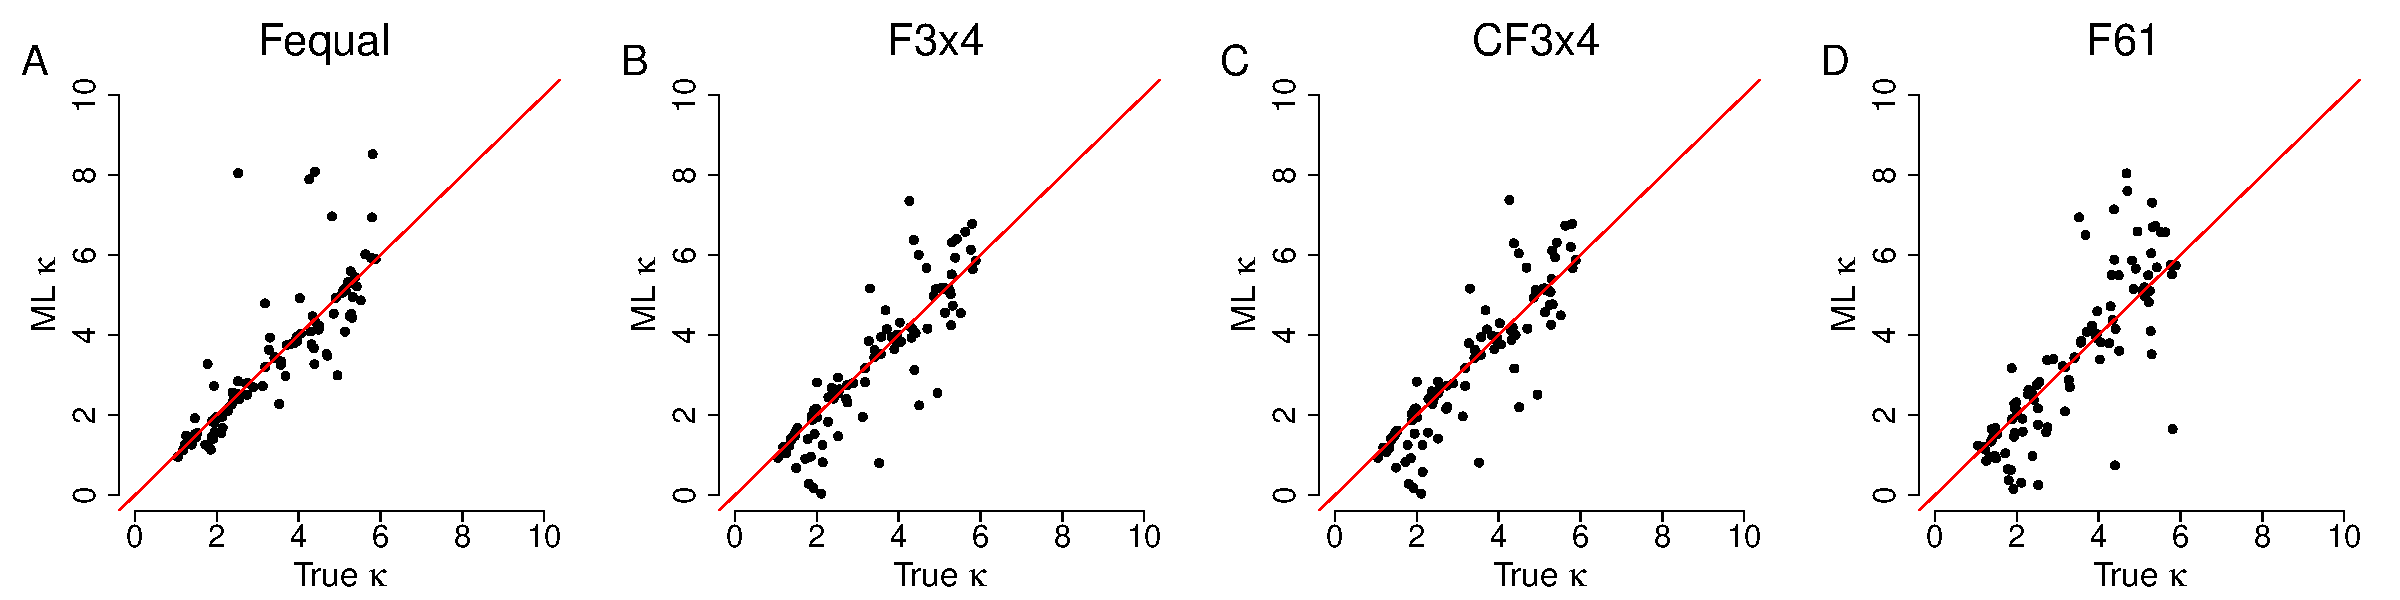
\includegraphics[width=6in]{figures/SI/regression_kappa_nobias.pdf}}
\noindent \textbf{Fig. S3} Kappa regression for all ML freqspec parameterizations where kappa is a free parameter, without codon bias.
\customlabel{fig:reg_kappa_nobias}{S3}

\bigskip
\bigskip
\bigskip


\centerline{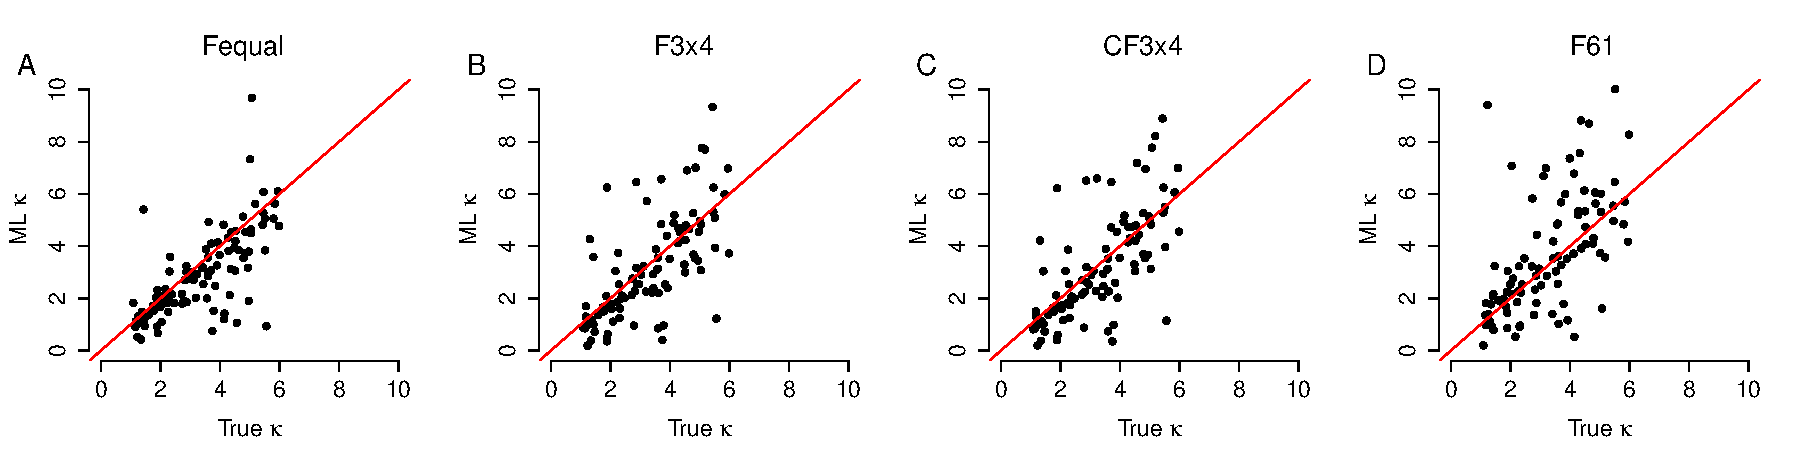
\includegraphics[width=6in]{figures/SI/regression_kappa_bias.pdf}}
\noindent \textbf{Fig. S4} Kappa regression for all ML freqspec parameterizations where kappa is a free parameter, without codon bias.
\customlabel{fig:reg_kappa_bias}{S4}


\end{document}

